\section{Strip}
\label{sec:strip}

\begin{figure}[h!] 
	\centering
	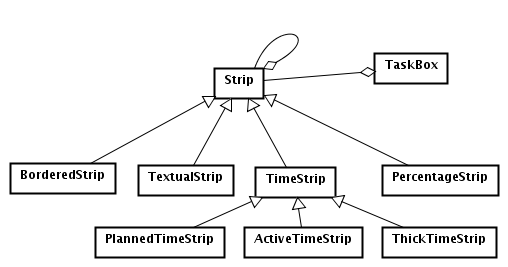
\includegraphics[width=0.7\textwidth]{../StripDetail.png}
	\caption{kinds of strips}
	\label{fig:strip} 
\end{figure}

La \emph{Strip} modella il concetto di ''striscia'': lo possiamo vedere come il
building block di pi\`u basso livello di tutta la nostra analisi. Si possono
osservare queste relazioni:
\begin{description}
  \item[TaskBox composition] \emph{TaskBox} contiene delle \emph{Strip},
  indipendentemente dalla rappresentazione dedicata ad uno specifico \emph{Chart}. Abbiamo costruito
  questa relazione in quanto per costruire un \emph{TaskBox} sar\`a sufficiente
  comporre un insieme di strip, tante quante sono necessarie per la corretta
  visualizzazione del \emph{Chart} che si sta disegnando.
  \item[russian doll] \emph{Strip} contiene a sua volta delle \emph{Strip}:
  questo \`e un concetto che pensiamo posso essere molto potente. Vogliamo rendere la
  \emph{Strip} un contenitore trasparente rispetto ad oggetti del suo stesso
  tipo. Questo ci permetter\`a di disegnare \emph{Strip} annidate, decidendo a
  runtime sia la \textbf{profondit\`a} di annidamento sia l'\textbf{ordine} con
  cui vengono annidate. Otteniamo cosi l'effetto di \emph{russian doll}, 
  dedicandoci a modellare solo alcune semplici specializzazioni di \emph{Strip},
  necessarie per l'implementazione delle notazioni richieste nel documento di specifica,
  limitandoci poi ad ottenere rappresentazioni complesse annidando quelle
  semplici.
  \item[specializations] abbiamo un primo livello di specializzazione:
  \begin{itemize}
    \item \emph{PercentageStrip} rappresenta un quantit\`a (l'intera
    \emph{Strip}) e la percentuale di comletamento (una parte di \emph{Strip}
    di colore diverso). Pu\`o essere composta da un \emph{GanttTaskBox} per
    indicare la percentuale di completamento relativa al \emph{Task}
    rappresentato.
    
    \item \emph{TextualStrip} permette di inserire delle stringhe di caratteri
    all'interno della \emph{Strip}. Questa possiamo utilizzarla ad esempio nel
    \emph{GanttChart} sulla destra della relativa \emph{TaskBox} per indicare
    l'effort oppure le risorse.
    
    \item \emph{BorderedStrip} permette di costruire un bordo, in modo che
    possiamo implementare la notazione per \emph{field} come richiesto per
    \emph{NodeTaskBox}
    
    \item \emph{TimeStrip} permettono di rappresentare informazioni relative a
    un intervallo di tempo. Queste sono i building blocks per
    \emph{GanttChart}. Possiamo specializzare ulteriormente questo concetto:
    \begin{itemize}
      \item \emph{PlannedTimeStrip} per costruire la parte superiore del
      \emph{GanttTaskBox} cdns
      \item \emph{ActualTimeStrip} per costruire la parte inferiore del
      \emph{GanttTaskBox} cdns      
      \item \emph{ThickTimeStrip} per costruire la parte superiore del
      \emph{GanttTaskBox} nel caso la rappresentazione sia di un
      \emph{ComposedTask} cdns
    \end{itemize}
  \end{itemize}
\end{description}
